% LaTeX Curriculum Vitae Template
%
% Copyright (C) 2004-2009 Jason Blevins <jrblevin@sdf.lonestar.org>
% http://jblevins.org/projects/cv-template/
%
% You may use use this document as a template to create your own CV
% and you may redistribute the source code freely. No attribution is
% required in any resulting documents. I do ask that you please leave
% this notice and the above URL in the source code if you choose to
% redistribute this file.

\documentclass[letterpaper]{article}
% \usepackage{kotex}
\usepackage[pdftex]{graphicx}

\usepackage{hyperref}
\usepackage{geometry}

\usepackage{revnum}

\usepackage{color}
\definecolor{LightGray}{rgb}{0.8,0.8,0.8}
\definecolor{DarkGray}{rgb}{0.4,0.4,0.4} 

% Comment the following lines to use the default Computer Modern font
% instead of the Palatino font provided by the mathpazo package.
% Remove the 'osf' bit if you don't like the old style figures.
\usepackage[T1]{fontenc}
\usepackage[sc,osf]{mathpazo}

\usepackage{longtable}

% Set your name here
\def\name{Sangho Lee}

% Replace this with a link to your CV if you like, or set it empty
% (as in \def\footerlink{}) to remove the link in the footer:
\def\footerlink{}

% The following metadata will show up in the PDF properties
\hypersetup{
  colorlinks = true,
  urlcolor = black,
  pdfauthor = {\name},
  pdfkeywords = {economics, statistics, mathematics},
  pdftitle = {\name: Curriculum Vitae},
  pdfsubject = {Curriculum Vitae},
  pdfpagemode = UseNone
}

\geometry{
  body={6.5in, 8.5in},
  left=1.0in,
  top=1.25in
}

% Customize page headers
\pagestyle{myheadings}
\markright{\name}
\thispagestyle{empty}

% Custom section fonts
\usepackage{sectsty}
\sectionfont{\rmfamily\mdseries\Large}
\subsectionfont{\rmfamily\mdseries\itshape\large}

% Other possible font commands include:
% \ttfamily for teletype,
% \sffamily for sans serif,
% \bfseries for bold,
% \scshape for small caps,
% \normalsize, \large, \Large, \LARGE sizes.

% Don't indent paragraphs.
\setlength\parindent{0em}

% Make lists without bullets
\renewenvironment{itemize}{
  \begin{list}{}{
    \setlength{\leftmargin}{1.5em}
  }
}{
  \end{list}
}

\begin{document}

% Place name at left
{\huge \name}

% Alternatively, print name centered and bold:
%\centerline{\huge \bf \name}

\vspace{0.25in}

% \begin{minipage}{0.15\linewidth}
% \includegraphics[width=\linewidth]{sangho2}
% % 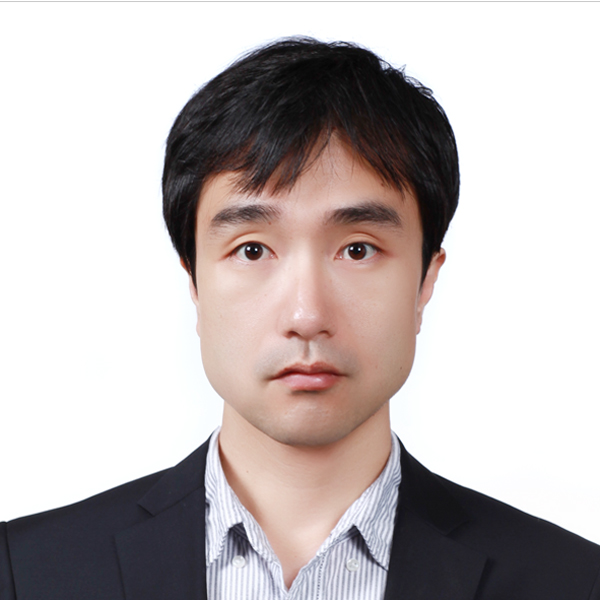
\includegraphics[width=1in,height=1.25in,clip,keepaspectratio]{sangho}
% \end{minipage}
% ~
\begin{minipage}{0.5\linewidth}
  Post-doctoral Research Associate \\
  Dept. of Computer Science \& Engineering \\
  \href{http://www.postech.ac.kr}{POSTECH} \\  
  Pohang, Republic of Korea
\end{minipage}
\begin{minipage}{0.5\linewidth}
  \begin{tabular}{ll}
    Phone:    & +82 54 279 2915 \\
    Fax:      & +82 54 279 1805 \\
    Email:    & {\tt sangho2@postech.ac.kr} \\
%               & {\tt sangho35.lee/@/gmail.com} \\
    % Homepage: & {\tt https://hpc.postech.ac.kr/$\sim$sangho2} \\
  \end{tabular}
\end{minipage}

\section*{Education}

\begin{itemize}
  \item Ph.D. in Computer Science and Engineering, POSTECH, February 2013.
  \item M.S. in Computer Science and Engineering, POSTECH, February 2008.
  \item B.S. in Computer Engineering, Hongik University, February 2006.
\end{itemize}

\section*{Career}
\begin{itemize}
  \item Post-doctoral Research Associate, POSTECH, from March 2013.
  \item Research Assistant, POSTECH, March 2006--February 2013.
\end{itemize}

\section*{Research Interests}
 %Information, Network, and System Security, Applied Cryptography
All aspects of computer security and privacy including Web and social network security, system security, and mobile security
% Web and social network security, applied cryptography, network security, system security

\section*{Referred Publications}
% \section*{Selected Publications}

% \item {\bf Sangho Lee} and Jong Kim, A batch rekeying time decision algorithm for large-scale IPTV
%   systems, {\it IEEE Transactions on Communications}, 2011. (In preparation)
% \item {\bf Sangho Lee}, Byoungyoung Lee, Jaehyeok Song, and Jong Kim, Detecting malicious pages
%   using passive analysis of URL shortening redirections, {\it Proceedings of 18th ACM Conference on
%     Computer and Communications Security (CCS)}, Chicago, IL, USA, October 17--21, 2011. (In
%   preparation)
%
% \begin{itemize}
% {\color{LightGray}
% \item {\bf Sangho Lee} and Jong Kim, Distributed URL shortening services, {\it Proceedings of 9th
%     USENIX Symposium on Networked Systems Design and Implementation (NSDI)}, Boston, MA, USA, March
%   30--April 1, 2012. (In preparation)
% \item {\bf Sangho Lee} and Jong Kim, Private retrieval of URL shortening services, {\it Proceedings
%     of 18th ACM Conference on Computer and Communications Security (CCS)}, Chicago, IL, USA, October
%   17--21, 2011. (In preparation)
% \item {\bf Sangho Lee}, Byoungyoung Lee, Jaehyeok Song, and Jong Kim, Detecting malicious pages
%   using passive analysis of URL shortening redirections, {\it Proceedings of 18th ACM Conference on \item[-] {\bf Sangho Lee} and Jong Kim, Distributed URL shortening services, {\it Proceedings of 9th

%     Computer and Communications Security (CCS)}, Chicago, IL, USA, October 17--21, 2011. (In
%   preparation)
% \item {\bf Sangho Lee} and Jong Kim, A muti-channel aware batch rekeying time decision algorithm for
%   IPTV systems, {\it IEEE Transactions on Communications}, 2011. (In preparation) }
% \item {\bf Sangho Lee} and Jong Kim, Privacy preserving URL shortening services, {\it Proceedings of
%     International World Wide Web Conference (WWW)}, 2012. (under review)
% {\color{DarkGray}
% \item \underline{\bf Sangho Lee} and Jong Kim, Detecting careless retweeters, {\it Proceedings of ACM
%     Conference on Computer and Communications Security (CCS)}, 2012. (in preparation)
% \item \underline{\bf Sangho Lee}, Jin Seok Kim, Sung Je Hong, and Jong Kim, Distance bounding with delayed responses,
%   {\it IEEE Communications Letters}, 2012. (under review)
% \item \underline{\bf Sangho Lee} and Jong Kim, Preserving source and sink location privacy in mission-critical
%   sensor networks, {\it Security and Communication Networks}. (under review)
% \item \underline{\bf Sangho Lee} and Jong Kim, Detection and analysis of malicious Twitter account names, {\it
%     Proceedings of USENIX Security Symposium}, 2012. (under review)
% }
% \end{itemize}
%
% \subsubsection*{Conference Papers}
\begin{longtable}{@{}p{0.8in}p{5.4in}@{}}
  TDSC'15 & Jonghyuk Song, {\bf Sangho Lee}, and Jong Kim, Inference Attack on Browsing History of Twitter Users using Public Click Analytics and Twitter Metadata, To appear in {\it IEEE Transactions on Dependable and Secure Computing}.\\\\
  \textbf{NDSS'15} & {\bf Sangho Lee}, Hyungsub Kim, and Jong Kim, Identifying Cross-origin Resource Status Using Application Cache, 
  To appear in {\em Proceedings of Network and Distributed System Security Symposium ({NDSS})}, San Diego, California, USA, February 8--11, 2015. \\\\
  \textbf{ACSAC'14} & Hyungsub Kim, {\bf Sangho Lee}, and Jong Kim, Exploring and Mitigating Privacy Threats of HTML5 Geolocation API, 
  {\em Proceedings of Annual Computer Security Applications Conference ({ACSAC})}, New Orleans, Louisiana, USA, December 8--12, 2014. \\\\
  COMCOM'14 & {\bf Sangho Lee} and Jong Kim, Early filtering of ephemeral malicious accounts on Twitter, 
  {\it Computer Communications} 54, 48--57, December 2014.\\\\
  \textbf{Oakland'14} & {\bf Sangho Lee}, Youngsok Kim, Jangwoo Kim, and Jong Kim, Stealing Webpages Rendered on Your Browser by Exploiting GPU Vulnerabilities, \emph{ Proceedings of IEEE Symposium on Security and Privacy ({Oakland})}, San Jose, California, USA, May 19--21, 2014.\\\\
  {WISA'13} & Hayoung Lee, Taeho Kang, {\bf Sangho Lee}, Jong Kim, and Yoonho Kim, Punobot: Mobile Botnet using Push Notification Service in Android, {\it Proceedings of International Workshop on Information Security Applications (WISA)}, Jeju Island, Korea, August 19--21, 2013.\\\\
  \textbf{WWW'13} & Jonghyuk Song, {\bf Sangho Lee}, and Jong Kim, I Know the Shortened URLs You Clicked on Twitter: Inference Attack using Public Click Analytics and Twitter Metadata, \emph{Proceedings of International World Wide Web Conference ({WWW})}, Rio de Janeiro, Brazil, May 13--17, 2013.\\\\
  TDSC'13 & {\bf Sangho Lee} and Jong Kim, WarningBird: A Near Real-time Detection System for Suspicious URLs in Twitter Stream, {\it IEEE Transactions on Dependable and Secure Computing}, 10(3), 183--195, May-June 2013.\\\\
  COMCOM'13 & {\bf Sangho Lee} and Jong Kim, Fluxing botnet command and control channels with URL shortening services, {\it Computer Communications} 36(3), 320--332, February 2013.\\\\
  COMML'12 & {\bf Sangho Lee}, Jin Seok Kim, Sung Je Hong, and Jong Kim, Distance Bounding with Delayed Responses, {\it IEEE Communications Letters} 16(9), 1478--1481, September 2012.\\\\
  JSS'12 & {\bf Sangho Lee}, Hay-Rim Lee, Seungkwang Lee, and Jong Kim, DRMFS: A file system layer for transparent access semantics of DRM-protected contents, {\it Journal of Systems and Software} 85(5), 1058--1066, May 2012.\\\\
  \textbf{NDSS'12} & {\bf Sangho Lee} and Jong Kim, WarningBird: Detecting Suspicious URLs in Twitter Stream, \emph{Proceedings of Network and Distributed System Security Symposium ({NDSS})}, San Diego, California, USA, February 5--8, 2012.\\\\
  \textbf{RAID'11} & Jonghyuk Song, {\bf Sangho Lee}, and Jong Kim, Spam Filtering in Twitter using Sender-receiver Relationship, \emph{Proceedings of International Symposium on Recent Advances in Intrusion Detection (\textbf{RAID})}, Menlo Park, California, USA, September 20--21, 2011.\\\\
  CCNC'11 & {\bf Sangho Lee} and Jong Kim, A Batch Rekeying Time Decision Algorithm for IPTV Systems, {\it Proceedings of 8th IEEE Consumer Communications and Networking Conference (CCNC)}, Las Vegas, Nevada, USA, January 9--12, 2011.\\\\
  ISCC'10 & {\bf Sangho Lee}, Heejin Park, and Jong Kim, A Secure and Mutual-profitable DRM Interoperability Scheme, {\it Proceedings of 15th IEEE Symposium on Computers and Communications (ISCC)}, Riccione, Italy, June 22--25, 2010.\\\\
  IJIS'09 & {\bf Sangho Lee}, Jong Kim, and Sung Je Hong, Redistributing time-based rights between consumer devices for content sharing in DRM system, {\it International Journal of Information Security} 8(4), 263--273, August 2009.\\\\
  JSS'09 & {\bf Sangho Lee}, Jong Kim, and Sung Je Hong,  Security weakness of Tseng's fault-tolerant conference-key agreement protocol, {\it Journal of Systems and Software} 82(7), 1163--1167, July 2009.\\\\
  BMSB'08 & Yuna Kim, Jae Keun Park, Hong Jun Choi, {\bf Sangho Lee}, Heejin Park, Jong Kim, Zino Lee, and Kwangil Ko, Reducing IPTV Channel Zapping Time based on Viewer's Surfing Behavior and Preference, {\it Proceedings of 2008 IEEE International Symposium on Broadband Multimedia Systems and Broadcasting (BMSB)}, Las Vegas, USA, Mar. 31--Apr. 2, 2008.
\end{longtable}

% \section*{Under Review}
% \begin{itemize}
% \item Beumjin Cho, {\bf Sangho Lee}, and Jong Kim, Self-collusion Attack: Privilege Escalation Through Application Update on Android.
% % , \emph{ Proceedings of IEEE Symposium on Security and Privacy ({Oakland})}, San Jose, California, USA, May 18--20, 2015.
% \item Hyungsub Kim, {\bf Sangho Lee}, and Jong Kim, Inferring Secrets from Storage Footprints through Quota Management API.
% % , \emph{ Proceedings of IEEE Symposium on Security and Privacy ({Oakland})}, San Jose, California, USA, May 18--20, 2015.
% \item {\bf Sangho Lee}, Jong Kim, and Yoonho Kim, Investigating Fake Friendships on Twitter.
% % , Computer Networks.
% \item {\bf Sangho Lee} and Jong Kim, Preserving Source- and Sink-location Privacy in Sensor Networks.
% % , Computer Science and Information Systems.
% \end{itemize}

% \begin{itemize}
% % \item Youngsok Kim, {\bf Sangho Lee}, Jangwoo Kim, and Jong Kim, CleanGPU: Precise deletion of sensitive data in GPU memory using static and dynamic lifetime prediction, {\it Proceedings of IEEE International Symposium on High Performance Computer Architecture (HPCA)}, 2014. (in preparation)
% % \item {\bf Sangho Lee}, Youngsok Kim, Jangwoo Kim, and Jong Kim, Fast and robust covert channels with GPU, {\it Proceedings of Network and Distributed System Security Symposium (NDSS)}, 2014. (under review)
% % \item {\bf Sangho Lee}, Hyungsub Kim, and Jong Kim, SpyCache: Scriptless Web privacy attacks using cross-origin application cache, {\it Proceedings of USENIX Security Symposium}, 2014. (under review)
% % \item Beumjin Cho, {\bf Sangho Lee}, and Jong Kim, Enforcing high-level Android permissions on low-level resources, {\it Proceedings of USENIX Annual Technical Conference (ATC)}, 2014. (under review)
% \item Hyungsub Kim, {\bf Sangho Lee}, and Jong Kim, Exploring and mitigating privacy threats of HTML5 geolocation API, {\em Proceedings of Annual Computer Security Applications Conference (\textbf{ACSAC})}, New Orleans, Louisiana, USA, December 8--12, 2014.
% \item {\bf Sangho Lee}, Youngsok Kim, Jangwoo Kim, and Jong Kim, Stealing webpages rendered on your browser by exploiting GPU vulnerabilities, \emph{ Proceedings of IEEE Symposium on Security and Privacy (\textbf{Oakland})}, San Jose, California, USA, May 19--21, 2014.
% \item Hayoung Lee, Taeho Kang, {\bf Sangho Lee}, Jong Kim, and Yoonho Kim, Punobot: Mobile botnet using push notification service in Android, {\it Proceedings of International Workshop on Information Security Applications (WISA)}, Jeju Island, Korea, August 19--21, 2013.
% \item Jonghyuk Song, {\bf Sangho Lee}, and Jong Kim, I know the shortened URLs you clicked on Twitter: Inference attack using public click analytics and Twitter metadata, \emph{Proceedings of International World Wide Web Conference (\textbf{WWW})}, Rio de Janeiro, Brazil, May 13--17, 2013.
% \item {\bf Sangho Lee} and Jong Kim, WarningBird: Detecting suspicious URLs in Twitter stream, \emph{Proceedings of Network and Distributed System Security Symposium (\textbf{NDSS})}, San Diego, California, USA, February 5--8, 2012.
% \item Jonghyuk Song, {\bf Sangho Lee}, and Jong Kim, Spam filtering in Twitter using sender-receiver relationship, \emph{Proceedings of International Symposium on Recent Advances in Intrusion Detection (\textbf{RAID})}, Menlo Park, California, USA, September 20--21, 2011.
% \item {\bf Sangho Lee} and Jong Kim, A batch rekeying time decision algorithm for IPTV systems, {\it Proceedings of 8th IEEE Consumer Communications and Networking Conference (CCNC)}, Las Vegas, Nevada, USA, January 9--12, 2011.
% \item {\bf Sangho Lee}, Heejin Park, and Jong Kim, A secure and mutual-profitable DRM interoperability scheme, {\it Proceedings of 15th IEEE Symposium on Computers and Communications (ISCC)}, Riccione, Italy, June 22--25, 2010. 
% \item Yuna Kim, Jae Keun Park, Hong Jun Choi, {\bf Sangho Lee}, Heejin Park, Jong Kim, Zino Lee, and Kwangil Ko, Reducing IPTV channel zapping time based on viewer's surfing behavior and preference,  {\it Proceedings of 2008 IEEE International Symposium on Broadband Multimedia Systems and Broadcasting (BMSB)}, Las Vegas, USA, Mar. 31--Apr. 2, 2008.
% \end{itemize}

% \subsubsection*{Journal Papers}
% \begin{itemize}
% %{\color{LightGray}
% % \item {\bf Sangho Lee} and Jong Kim, Self colluding attack: Malicious activities across application updates in Android, {\it Proceedings of Network and Distributed System Security Symposium (NDSS)}, 2014. (in preparation)
% % \item {\bf Sangho Lee} and Jong Kim, SpamMonitor: Monitoring the possible spam targets on Twitter, {\it Proceedings of Network and Distributed System Security Symposium (NDSS)}, 2014. (in preparation)
% %  \item Jaehyung Ahn, Hayoung Lee, {\bf Sangho Lee}, Jangwoo Kim, and Jong Kim, SafePush: Securing push notification service through dynamic permission check, {\it Proceedings of ACM Conference on Computer and Communications Security (CCS)}, 2013. (in preparation)
% % }
% % {\color{DarkGray}
% % }
% % \item Jonghyuk Song, {\bf Sangho Lee}, and Jong Kim, Inference attack on browsing history of Twitter users using public click analytics and Twitter metadata, \emph{IEEE Transactions on Dependable and Secure Computing}. (under review)
% % \item {\bf Sangho Lee} and Jong Kim, Preserving source- and sink-location privacy in sensor networks, {\it INFORMATION-An International Interdisciplinary Journal}. (under review)
% \item {\bf Sangho Lee} and Jong Kim, Early filtering of ephemeral malicious accounts on Twitter, To appear in {\it Computer Communications}.
% \item {\bf Sangho Lee} and Jong Kim, WarningBird: A near real-time detection system for suspicious URLs in Twitter stream, {\it IEEE Transactions on Dependable and Secure Computing}, 10(3), 183--195, May-June 2013.
% \item {\bf Sangho Lee} and Jong Kim, Fluxing botnet command and control channels with URL shortening services, {\it Computer Communications} 36(3), 320--332, February 2013.
% \item {\bf Sangho Lee}, Jin Seok Kim, Sung Je Hong, and Jong Kim, Distance bounding with delayed responses, {\it IEEE Communications Letters}, 16(9), 1478--1481, September 2012.
% \item {\bf Sangho Lee}, Hay-Rim Lee, Seungkwang Lee, and Jong Kim, DRMFS: A file system layer for transparent access semantics of DRM-protected contents, {\it Journal of Systems and Software} 85(5), 1058--1066, May 2012.
% %\item {\bf Sangho Lee} and Jong Kim, Detecting suspicious URLs in Twitter stream (poster), {\it
% %    USENIX Security Symposium}, San Francisco, California, USA, August 8--12, 2011.
% % \item Hay-Rim Lee, {\bf Sangho Lee}, Jihun Kim, Sung Je Hong, and Jong Kim, Self-detection of packet
% %   misrouting nodes for MANET with AODV, {\it Proceedings of 2011 International Symposium on Embedded
% %     Technology (ISET)}, Jeju Island, Korea, May 20--21, 2011.

% \item
%  {\bf Sangho Lee}, Jong Kim, and Sung Je Hong, 
%  Redistributing time-based rights between consumer devices for content sharing in DRM system,
%  {\it International Journal of Information Security} 8(4), 263--273,
%  August 2009.
% \item 
%  {\bf Sangho Lee}, Jong Kim, and Sung Je Hong, 
%  Security weakness of Tseng's fault-tolerant conference-key agreement protocol,
%  {\it Journal of Systems and Software} 82(7), 1163--1167,
%  July 2009.
% \end{itemize}

% \subsubsection*{Domestic Journal Paper}
% \begin{itemize}
% \item
%  {\bf Sangho Lee}, Jong Kim, and Sung Je Hong,
%  Efficient fault-tolerant conference-key agreement using ID-based one round tripartite key agreement protocol, 
%  {\it Journal of KIISE : Computing Practices and Letters}, vol. 14(5), 512--516, 
%  July 2008 (text in Korean).
% \end{itemize}

% \subsubsection*{Domestic Conference Papers}
% \begin{itemize}
% \item 
%  Heejin Park, {\bf Sangho Lee}, and Jong Kim,
%  Rights preserving interoperability protocol in DRM,
%  {\it Proceedings of 2008 KIISC Winter Conference}, vol. 18(2), 141--144, Seoul, Korea,
%  December 2008 (text in Korean).
% \item
%  {\bf Sangho Lee}, Yuna Kim, Jong Kim, and Zino Lee, 
%  Program-value aware adaptive group-key rekeying for IPTV,
%  {\it Proceedings of 2008 KIPS Fall Conference}, vol. 15(2), 1437--1440, Seoul, Korea,
%  November 2008 (text in Korean).
% \item
%  {\bf Sangho Lee}, Jong Kim, and Sung Je Hong, 
%  Efficient fault-tolerant conference-key agreement based on ID-based tripartite key agreement protocol,
%  {\it Proceedings of 2007 KIISE Fall Conference}, vol. 34(2A), 104--105, Busan, Korea, 
%  October 2007 (text in Korean).
% \end{itemize}

\section*{Thesis}
\begin{itemize}
 \item
 {\bf Sangho Lee},
 Detection and Prevention of Web Security Attacks Exploiting URL Redirection,
 Doctoral Thesis, Department of Computer Science and Engineering, POSTECH, 
 February 2013.
 \item
 {\bf Sangho Lee},
 Redistributing Time-based Rights for Content Sharing in DRM, 
 Master's Thesis, Department of Computer Science and Engineering, POSTECH, 
 February 2008.
\end{itemize}

\section*{Patents}
\begin{itemize}
  \item
 Jong Kim, {\bf Sangho Lee}, and Heejin Park,
 Methods and apparatuses for providing DRM interoperability,
 Registration, USA, 8,386,799,
 February 2013. 
 \item
 {\bf Sangho Lee} and Jong Kim,
 Method of distributing time of using contents between personal devices and system based on the same,
 Registration, Korea, 10-0951792,
 April 2010.
  \item
 Heejin Park, Jong Kim, and {\bf Sangho Lee},
 Method and apparatus for rights-preserving interoperability in DRM,
 Registration, Korea, 10-0942992
 February 2010. 
\end{itemize}

\section*{Projects}

\begin{itemize}
 \item January 2010--December 2011: Research on the context-aware privacy protection platform for mobile device, ITRC-CMEST
 \item February 2010--April 2011: Research on embedded system vulnerabilities, Samsung Electronics
 \item March 2006--December 2009: Research on the DRM middleware for mobile device, ITRC-CMEST.
 \item March 2007--November 2008: Research on the security of IPTV system, Contron and Alticast.
 \item September 2007--February 2008: Survey on the sensors and industrial applications of USN, SECUI.COM.
 \item March 2006--October 2006: Research on the detection rule optimization for improving IDS engine, NSRI.
\end{itemize}

% \section*{Academic Experience}

% \begin{itemize}
%  \item Teaching Assistant, Data Structures, POSTECH, Fall 2007.
% \end{itemize}

\section*{Honors and Awards}

\begin{itemize}
 \item Runner-up Prize, Evaluation of ITRC Support Program, 2013.
 \item Good Paper Award, KIISC Winter Conference, 2008.
 \item Good Paper Award, KIISE Fall Conference, 2007.
 % \item Best Grade Scholarship, Hongik University, from 2002 to 2006.
\end{itemize}

\section*{Professional Activities}

\begin{itemize}
% \item External reviewer for WWW, ICDCS, NDSS, IEEE Trans. Dependable and Secure Computing, IEEE Communications Letters, and Wiley Security and Communication Networks
\item External/Sub reviewer for ICDCS, WWW, NDSS, IEEE Communications Letters, IEEE Trans. Dependable and Secure Computing, and Wiley Security and Communication Networks
% \item Student Member of IEEE
\end{itemize}

\section*{Talks}

\begin{itemize}
\item Identifying Cross-origin Resource Status Using Application Cache, {\it 22nd Network and 
    Distributed System Security Symposium (NDSS)}, San Diego, California, USA, February 9, 2015.
\item Web and Browser Security: Attack and Defense, {\it Invited Seminar}, UNIST, Ulsan, Korea, January 21, 2015.
\item Stealing Webpages Rendered on Your Browser by Exploiting GPU Vulnerabilities, {\it 35th IEEE Symposium on Security and Privacy (Oakland)}, San Jose, California, USA, May 19, 2014.
% \item Distributed certificate authority scheme with weighted secret sharing for mobile ad-hoc networks, {\it 4th International Conference on Network of the Future (NoF)}, Pohang, Korea, October 24, 2013.
\item Spam and Browsing Privacy Problems on Twitter, {\it Invited Seminar}, KAIST, Daejeon, Korea, May 27, 2013.
\item WarningBird: Detecting Suspicious URLs in Twitter Stream, {\it 19th Network and 
    Distributed System Security Symposium (NDSS)}, San Diego, California, USA, February 8, 2012.
\item A Batch Rekeying Time Decision Algorithm for IPTV Systems, {\it 8th IEEE Consumer
    Communications and Networking Conference (CCNC)}, Las Vegas, Nevada, USA, January 11, 2011.
\item A Secure and Mutual-profitable DRM Interoperability Scheme, {\it 15th IEEE Symposium on
    Computers and Communications (ISCC)}, Riccione, Italy, June 22, 2010.
\item Program-value aware Adaptive Group-key Rekeying for IPTV, {\it KIPS Fall Conference}, Seoul,
  Korea, November 15, 2008.
\item Efficient Fault-tolerant Conference-key Agreement based on ID-based Tripartite Key Agreement
  Protocol, {\it KIISE Fall Conference}, Busan, Korea, October 27, 2007.
\item DRM-enabled Adaptive User Domain using Time-block Redistribution, {\it 5th Joint Workshop
    between Security Research Labs in Korea and Japan}, Hakodate, Japan, August 4, 2007.
\item Controlled Content Sharing based on Time-block Distribution in DRM, {\it 4th Joint Workshop
    between Security Research Labs in Korea and Japan}, Pohang, Korea, January 29, 2007.
\end{itemize}

% \begin{minipage}{0.15\linewidth}
% \includegraphics[width=\linewidth]{sangho2}
% % 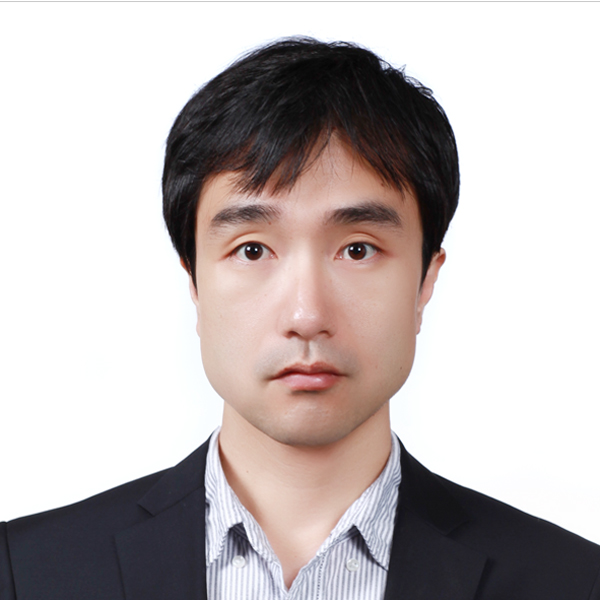
\includegraphics[width=1in,height=1.25in,clip,keepaspectratio]{sangho}
% \end{minipage}
% ~
% \begin{minipage}{0.5\linewidth}
%   Post-doctoral Research Associate \\
%   Dept. of Computer Science \& Engineering \\
%   \href{http://www.postech.ac.kr}{POSTECH} \\  
%   Pohang, Republic of Korea
% \end{minipage}
% \begin{minipage}{0.5\linewidth}
%   \begin{tabular}{ll}
%     Phone:    & +82 54 279 2915 \\
%     Fax:      & +82 54 279 1805 \\
%     Email:    & {\tt sangho2@postech.ac.kr} \\
% %               & {\tt sangho35.lee/@/gmail.com} \\
%     % Homepage: & {\tt https://hpc.postech.ac.kr/$\sim$sangho2} \\
%   \end{tabular}
% \end{minipage}

% \section*{References}
% \begin{minipage}{0.33\linewidth}
% Prof. Jong Kim\\
% POSTECH\\
% Nam-gu, Pohang-si\\
% Gyeongsangbuk-do, Korea\\
% +82 54 279 2257\\
% {\tt jkim@postech.ac.kr}
% \end{minipage}
% ~
% \begin{minipage}{0.33\linewidth}
% Prof. Jangwoo Kim\\
% POSTECH\\
% Nam-gu, Pohang-si\\
% Gyeongsangbuk-do, Korea\\
% +82 54 279 2390\\
% {\tt jangwoo@postech.ac.kr}
% \end{minipage}
% ~
% \begin{minipage}{0.33\linewidth}
% Dr. Jin Seok Kim\\
% Agency for Defense Development\\
% Jinhae-gu, Changwon-si\\
% Gyeongsangnam-do, Korea\\
% +82 55 540 6218\\
% {\tt treasure@add.re.kr}
% \end{minipage}

\bigskip

% Footer
\begin{center}
  \begin{footnotesize}
    Last updated: \today \\
    \href{\footerlink}{\texttt{\footerlink}}
  \end{footnotesize}
\end{center}

\end{document}
